% Mon premier fichier avec LaTeX.
% Ceci est un commentaire.
% Type de document : "article"
\documentclass{article}
%----- préambule ---------
% Encodage du fichier source
\usepackage[utf8]{inputenc}
% Typographie française
%\usepackage[français]{babel}
% Utile pour les figures
\usepackage{graphicx}
% déclarations pour l’en-tête
\title{TP3 Ingeniérie logicielle en \LaTeX}
\author{AUDIC Bryan \& NAPOLEON Sebastien}
%---- corps --------
\begin{document}
\maketitle
\section{Insertion d'une image}
Voici l'image créée sous Inkscape :
\begin{center}

\includegraphics[width=3cm]{figure.eps}
\end{center}
\section{Partie 1.2}
\paragraph{Question 3 : graphe des dépendances}
\begin{center}
\includegraphics[width=10cm]{dependance.eps}
\end{center}
\paragraph{Question 4 : Premier Makefile}
\begin{verbatim}
all : foo.pdf clean

foo.pdf : foo.dvi
	dvipdf foo.dvi
foo.dvi : foo.tex figure.eps dependance.eps
	latex foo.tex
clean : 
	rm -rf foo.aux foo.log
\end{verbatim}
\paragraph{Question 5 : Comportement Makefile}
1 - Pas de nouvelle compilation.
2 - Après utilisation du touch, la compilation s'effectue à nouveau car l'horodatage a changé.
3 - La compilation s'effectue car le .tex est plus récent que le .dvi alors que le .pdf est plus récent que le .tex. Cela s'explique par le fait que le systeme de makefile remonte la chaine de dépendance et ne s'arrête pas seulement au début. Ainsi, le .tex est recompilé et le .dvi est devenu obsolète. Même chose pour le .dvi et le .pdf.
\section{Partie 1.3}
\paragraph{Question 6 : Règle Makefile}
\begin{verbatim}
all : pdf clean

pdf : foo.dvi
	dvipdf foo.dvi
foo.dvi : foo.tex figure.eps dependance.eps
	latex foo.tex
dvi : foo.dvi
	xdvi foo.dvi
clean : 
	rm -rf foo.aux foo.log
\end{verbatim}
A partir d'ici, nous n'avons pas eu le temps de modifier le reste du code pour y ajouter le foo.dvi partout. Normalement il faudrait cette étape intermédiaire pour diffencier la compilation du .tex et l'affichage du .dvi.
Le code dans le reste du fichier est fonctionnel.
\paragraph{Question 7 : Macro}
\begin{verbatim}
#MACROS
LATEX=latex
BASENAME=foo
DVItoPDF=dvipdf
DPFLAGS=
VIEWER=xdvi
PDFVIEWER=evince

#REGLES
all : pdf clean

pdf : dvi
	$(DVItoPDF) $(BASENAME).dvi
dvi : $(BASENAME).tex figure.eps dependance.eps
	$(LATEX) $(BASENAME).tex
	$(VIEWER) $(BASENAME).dvi
clean : 
	rm -rf $(BASENAME).aux $(BASENAME).log
\end{verbatim}
\paragraph{Question 8 : Macros spéciales}
\begin{verbatim}
#MACROS
LATEX=latex
BASENAME=foo
DVItoPDF=dvipdf
DPFLAGS=
VIEWER=xdvi
PDFVIEWER=evince

#REGLES
all : pdf clean

pdf : dvi
	$(DVItoPDF) $(BASENAME).$<
dvi : $(BASENAME).tex figure.eps dependance.eps
	$(LATEX) $<
	$(VIEWER) $(BASENAME).$@
clean : 
	rm -rf $(BASENAME).aux $(BASENAME).log
\end{verbatim}
\paragraph{Question 9-10 : Makefile générique}
\begin{verbatim}
#MACROS
LATEX=latex
BASENAME=foo
DVItoPDF=dvipdf
DPFLAGS=
VIEWER=xdvi
PDFVIEWER=evince

#REGLES
#all : pdf clean
%.pdf : %.dvi
	$(DVItoPDF) $<
%.dvi : %.tex figure.eps dependance.eps
	$(LATEX) $<
	$(VIEWER) $@
clean : 
	rm -rf $(BASENAME).aux $(BASENAME).log

help :
	@echo "	nomDuFichier.dvi : Genere le dvi associer a un fichier tex et l'affiche."
	@echo "	nomDuFichier.pdf : Genere le pdf associer a un fichier dvi."
	@echo "	clean : Supprime les fichiers .aux .log."
\end{verbatim}

\section{Partie 1.4}
\paragraph{Question 11 : Compilation en C}
La direcive défault sert à indiquer un message en cas de cible incorrect pour la commande make.
La valeur de OBJS est : hello-world.o car on substitue le .c par .o.
La règle de construction de l'application, après substitution, est : 
gcc  hello-world.o -o hello-world 

\paragraph{Question 12 : Suffixes en C}
Il y a une erreur car que le .o n'existe pas.
Si on met .SUFFIXES en commentaire, les suffixes ne sont pas supprimés par défaut et donc conservés. Donc la compilation fonctionne.

\paragraph{Question 13 : Création d'un fichier compressé}
\begin{verbatim}
APPL = hello-world

SHELL = /bin/sh

# paramètres de compilation et d'édition de liens
CC = gcc
LD = $(CC)
CFLAGS =
LDFLAGS =
CPPFLAGS =
LOADLIBS =
LDLIBS =
TAROPT=zcvf

# objets de l'application
SRCS = hello-world.c 
OBJS = $(subst .c,.o,$(SRCS))
EXEC = $(APPL)

# directive d'inhibition des suppressions
.PRECIOUS: $(EXEC)

# directive d'action par défaut, en cas d'erreur
.DEFAULT: ; @echo "$< n'est pas une cible valide"
	
# directive d'application des règles implicites
.SUFFIXES:             # supprime les suffixes par défaut
#.SUFFIXES: .c .o      # définit une liste de suffixes

%.o : %.c
	$(CC) -c $(CFLAGS) $(CPPFLAGS) $< -o $@


		  
# règle de construction de l'application
$(EXEC): $(OBJS)
	$(LD) $(LDFLAGS) $^ -o $@ $(LOADLIBS) $(LDLIBS)

$(APPL).tar.gz: $(OBJS)
	tar $(TAROPT) $@ $(APPL)

clean:
	-@rm -f $(OBJS) $(EXEC) core a.out 2>/dev/null
\end{verbatim}

\end{document}
%---- fin du corps